\chapter{Quality Measures}\label{quality-measures}

In order to ensure proper quality a number of measurements were taken. The following section describes every measurement separately.

\section{Testing}\label{testing}

OSM2VectorTiles consists of many different components that all work together which makes testing quite challenging. This section describes how testing was approached in this project.

\subsection{Mapping Report Tool}

The Mapping Report tool was created to verify that all imported \osm{} data is used inside the vector tiles. This helped to identify \osm{} key/value pairs which should be removed from the import mapping because they are not used inside the vector tiles.

\begin{table}[H]
\centering
\begin{tabular}{llrrr}
\hline
OSM Tables             & Vector Tile Layers    & All Records & \multicolumn{1}{l}{Used Records} & \multicolumn{1}{l}{Percent} \\ \hline
osm\_admin\_*          & admin                 & 11284       & 813                              & 7.2                         \\
osm\_aero\_*           & aeroway               & 643         & 643                              & 100                         \\
osm\_airport\_*        & airport\_label        & 199         & 199                              & 100                         \\
osm\_barrier\_*        & barrier\_line         & 22880       & 22880                            & 100                         \\
osm\_building\_*       & building              & 604304      & 604304                           & 100                         \\
osm\_housenumber\_*    & housenum\_label       & 108376      & 108376                           & 100                         \\
osm\_landuse\_*        & landuse (overlay)     & 79337       & 79337                            & 100                         \\
osm\_mountain\_peak\_* & mountain\_peak\_label & 3235        & 3235                             & 100                         \\
osm\_place\_*          & place\_label          & 12269       & 6921                             & 56.41                       \\
osm\_poi\_*            & poi\_label            & 120793      & 75108                            & 62.18                       \\
osm\_rail\_station\_*  & rail\_station\_label  & 2990        & 2990                             & 100                         \\
osm\_road\_*           & road (label)          & 522469      & 522469                           & 100                         \\
osm\_water\_linestring & waterway (label)      & 31075       & 20458                            & 65.83                       \\
osm\_water\_polygon    & water (label)         & 10496       & 10496                            & 100                        
\end{tabular}
\caption{Example output of Mapping Report Tool}
\label{mapping_report_tool}
\end{table}

\autoref{mapping_report_tool} shows an example output of the Mapping Report Tool. It lists the number of rows per table and compares them with the number of rows used in a certain layer. If the percentage value is below 100 percent, the layer does not use all the features specified in the import mapping. Therefore these \osm{} key/value pairs should be removed.

\subsection{Integration Test}

In Travis CI\cite{pm_5_travis-ci.org_2015} the entire workflow was completed for a small data sample on each commit.
Because the entire workflow is configured with Docker Compose \cite{pm_6_docs.docker.com_2015} the CI server had to execute all import steps in serial order. This is a straightforward way to check if all components work together correctly
and although it is a simple setup it has helped tremendously during project development, catching bugs
like missing tables or SQL typos.

\begin{yamlcode}
script:
  # Test import
  - docker-compose up -d postgis
  - sleep 10
  - docker-compose run import-external
  - docker-compose run import-osm
  - docker-compose run import-sql
  # Test export
  - docker-compose run export
  # Test changed tiles
  - docker-compose run update-osm-diff
  - docker-compose run import-osm-diff
  - docker-compose run changed-tiles
\end{yamlcode}

\subsection{Structural Test}

The Vector Tile Compare tool was created to analyze the content of single vector tiles. This helped to identify which type of data is shown on which zoom levels and later to ensure that the same amount of features are present in OSM2VectorTiles compared to Mapbox Streets v7.

\subsection{Visual Test}

In addition to comparing the content of the vector tiles the Visual Compare tool was created to visually preview and compare the map on different zoom levels. 

\begin{figure}[H]
  \centering
  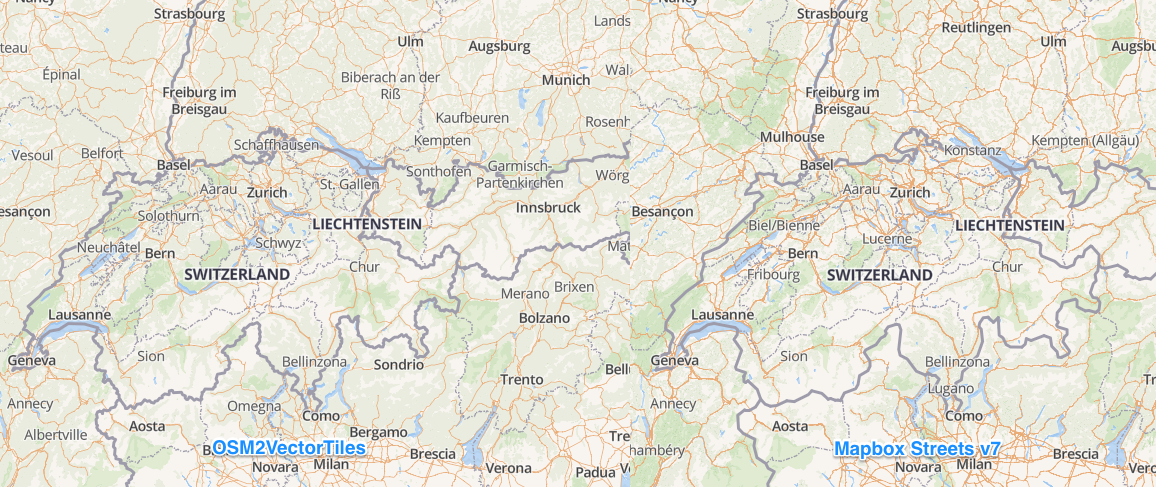
\includegraphics[width=1.0\textwidth]{images/visual_compare}
  \caption{Visual Compare Tool}
  \label{visual_compare} 
\end{figure}

\autoref{visual_compare} shows a screenshot of the Visual Compare tool. On the left hand side is OSM2VectorTiles and on the right hand side Mapbox Streets v7. Both use the OSM Bright visual style.

\section{Guidelines}\label{guidelines}
To have homogeneous software the contributors have settled on common guidelines in the beginning of the project.

\subsection{Releases}
Semantic versioning \cite{pm_7_preston-werner_2015} should be used for releases.
At the end of each milestone a new release will be created. For each release a changelog with all closed issues, merged pull requests and fixed bugs should be created. This makes it easier for people to track the progress of the project.

\subsection{Git}\label{git}
\paragraph{Commit Messages}
The seven rules of great git commit
messages\cite{pm_8_chris.beams.io_2015} should be used.

\paragraph{Rewriting}
Git history should be kept clean and therefore local branches should be squashed meaningfully.

\paragraph{Pulling}
To avoid unnecessary merge messages one should always use the
\texttt{-\/-rebase} parameter.

\subsection{Workflow}\label{git-workflow}
The Feature Branch Workflow\cite{pm_9_atlassian_git_tutorial_2015} should be used. Every project member has a local repository with a copy of the remote
repository. For each feature ticket in GitHub a separate branch
will be created. Once a ticket has been completed a pull request will be
created and needs to be reviewed and merged into the \texttt{master} branch by an other member.

\subsection*{Coding Standards}

\paragraph{Bash} Bash was used for the Docker image entrypoints and follow
the rules of Defensive Bash Programming \cite{pm_10_lavi_2012}.

\paragraph{Python} Python code should stay PEP-8\cite{pm_11_python.org_2015} compliant and write idiomatic Python code according to PEP-20\cite{pm_12_python.org_2015}.

\paragraph{JavaScript} The JavaScript code is checked using ESLint\cite{pm_13_eslint.org_2015}

\paragraph{SQL} The PostgreSQL code is using upper case for the key words. Apart from nice formatted SQL code and functions should be used
to keep the queries DRY\cite{pm_14_wikipedia_2015}.

\paragraph{Dockerfile} Dockerfiles follow the best practices\cite{pm_15_docs.docker.com_2015} defined by Docker.
